\documentclass[12pt]{article}

\usepackage{amsmath}

\usepackage{amssymb}

\usepackage{graphicx}

\usepackage{tikz}

\usetikzlibrary{quantikz}

\usepackage{hyperref}

\usepackage[utf8]{inputenc}

\title{Variational Quantum Classifiers}

\begin{document}

\maketitle

\tableofcontents

\section{Overview}
    Quantum machine learning, in the context being discussed, is typically just expressed as 
    a quantum circuit framework that processes and produces output for classical data sources. This is 
    desirable because classical machine learning takes a large number of computational resources to accomplish 
    a viable output. While the toll of methods such as gradient descent may be decreased with strategies like stochastic
    gradient descent, which is able to produce an output faster in certain cases, these results are not always guaranteed;
    quantum computing provides a strategy with which we can accomplish machine learning more effectively.

    \subsection{Goals}
        The goal of a variational classifier is simple; we take in a set of data, send it through a parameterized operation 
        that is then trained by an optimizer. The fundamental circuit is shaped of 
        simple, differentiated components that feed each other inputs from their own outputs.

    \subsection{Circuit Framework}
        \begin{center}
            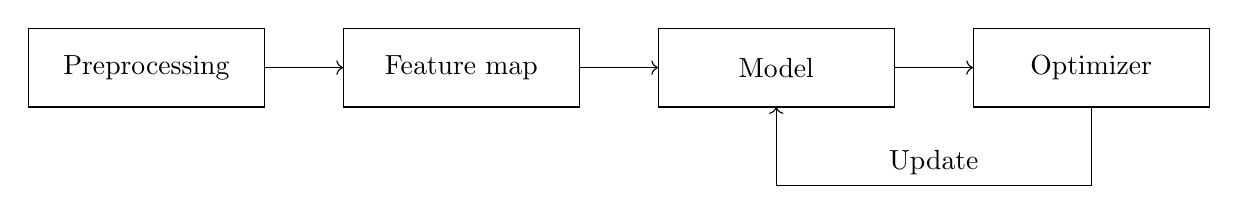
\begin{tikzpicture}
                \draw (0, 0) rectangle(3, 1);
                \draw (1.5, 0.5) node {Preprocessing};
                \draw [->] (3, 0.5) -- (4, 0.5);
                \draw (4, 0) rectangle(7, 1);
                \draw (5.5, 0.5) node {Feature map};
                \draw [->] (7, 0.5) -- (8, 0.5);
                \draw (8, 0) rectangle(11, 1);
                \draw (9.5, 0.5) node {Model};
                \draw [->] (11, 0.5) -- (12, 0.5);
                \draw (12, 0) rectangle(15, 1);
                \draw (13.5, 0.5) node {Optimizer};
                \draw (13.5, 0) -- (13.5, -1);
                \draw (13.5, -1) -- (9.5, -1);
                \draw [->] (9.5, -1) -- (9.5, 0);
                \draw (11.5, -0.7) node {Update};
            \end{tikzpicture}
        \end{center}
    
\section{Preprocessing}
    All that is required with preprocessing is to obtain a reliable data set 
    and organize it into a usable format. This is achieved through classical means by 
    filtering out entries by certain criteria such that the training data set is optimal 
    to use. In any regular dataset, the features can be ranked with respect to its correlation with the target
    variable; this will allow us to choose the most relevant features of the dataset to represent as a quantum state.

\section{State Preparation}
    In order to allow a quantum circuit to work with classical data, one must encode the data into a 
    quantum state that can be utilized by the quantum computer. The way this task can be achieved is through data embedding; moving classical 
    data into a quantum state in Hilbert space so that it can be accessed and used by the quantum computer.

    \subsection{Feature Map}
        A feature map is a construct that allows the embedding of data into higher-dimensional spaces (or quantum states). 
        It is modeled as a parametrized quantum circuit, where the inputs correspond to the parameters in the operation. 
        Effectively, what we want is some data point vector $\overrightarrow{x}$ to correspond:
        \[\overrightarrow{x} \to |\phi(\overrightarrow{x})\rangle\]
        where $\phi$ denotes some function on a ground state qubit that is parametrized by the original data point.
        In general terms, a feature map $\phi$ performs:
        \[\phi: \mathbb{R}^N \to \mathbb{C}^{2^n}\]
        The basic motivation behind the usage of a feature map is that nonlinear operations that are typically desired when encoding 
        data for machine learning purposes are hard to realize in a strongly linear system like quantum computing; the feature map shifts the burden of 
        producing nonlinearity into the procedure of encoding classical inputs to a quantum state. 

    \subsection{Basic Embedding}
        The most naive of embedding schemes, basic embedding simply associates each binary input with a bit-wise translation 
        of the input into corresponding states in the quantum system. The bitstring $x=101$, for example, can be expressed with 
        three qubits in a quantum circuit as the state $|101\rangle$. If we have a dataset $\mathcal{D}$ containing $M$ entries with $N$ bits for each entry, then the 
        entry $x$ can directly be mapped to $|x\rangle$. 
        The dataset can be represented in such a superposition:
        \[|\mathcal{D}\rangle = \frac{1}{\sqrt{M}} \sum^{M}_{m=1} |x^{(m)}\rangle\]
        However, for $N$ bits, there are $2^N$ possible states; we are wasting a lot of possible bit-space by using basic embedding.

    \subsection{Amplitude Embedding}
        In the amplitude encoding scheme, data from each entry is encoded into the amplitudes of a quantum state. 
        By normalizing the $N$-dimensional vector entry $x$, it can be represented by the amplitudes of a quantum state $|\psi_x\rangle$:
        \[|\psi_x\rangle = \sum_{i=1}^N x_i |i\rangle\]
        Note that $x_{norm} = 1$; this condition must be fulfilled for the state to be a valid quantum encoding.
        Considering the dataset $\mathcal{D}$, the amplitude embedding can be understood as a concatenation of the inputs $x^{(m)}$ into one vector:
        \[C = A\langle x_1^{(1)}, \cdots x_N^{(1)}, x_1^{(2)}, \cdots x_N^{(2)}, \cdots \rangle\]
        where $A$ represents the constant that normalizes the vector. The input is understood in the computational basis as 
        \[|\mathcal{D}\rangle = \sum_{i=1}^{2^n}C_i|i\rangle\]

        In our approach, we will require that the size of the input $N$ is a power of 2 so that we may associate it directly with an 
        amplitude vector in the computational basis. If $N$ is not a power of 2, we can add supplementary entries that pad the original input. We 
        can denote these with $c_1, c_2, \cdots c_D$, in which all of them are 0. So, we can transform 
        \[(x_1, \cdots x_N) \to A(x_1, \cdots x_N, c_1, \cdots c_D)\]
        where $A$ is the normalization factor,
        \[A = \frac{1}{\sqrt{\sum_j^N x^2_j + \sum_k^D |c_k|^2}}\]

\section{Variational Circuit}
    After the data encoding, we move on to the actual variational circuit. This circuit is some sort of block operator that 
    depends on a set of parameters, denoted within this writeup as a vector $\overrightarrow{\theta}$.
    There exist many different types of variation circuits, but many of them are similar in structure to another; they have specific components
    that work to achieve similar results.
    Typically, the variational circuit consists of parameterized rotation gates about some axis; in sticking to the real domain, the $R_y$ gate will be used. Then,
    entanglement gates are applied such that most of the qubits are connected in some way to each other. The block can then be repeated some number of times to 
    introduce more parameters into the model.
    In essence, the basic circuit looks like:
    \begin{center}
        \begin{quantikz}
            \lstick{\ket{0}} & \gate{R_y(\theta_0)} & \ctrl{1} & \qw      & \qw  & \qw & \rstick{\ldots}\\
            \lstick{\ket{0}} & \gate{R_y(\theta_1)} & \targ{}  & \ctrl{1} & \qw & \qw & \rstick{\ldots}\\
            \lstick{\ldots}  & \gate{\ldots} &        \qw      & \targ{} & \ctrl{1} & \qw & \rstick{\ldots}\\
            \lstick{\ket{0}} & \gate{R_y(\theta_n)} & \qw      & \qw     & \targ{} & \qw & \rstick{\ldots}
        \end{quantikz}
    \end{center}

\section{Classification}
    In between the circuit and the optimizer, we must somehow measure and classify our quantum data into a form that can be broken down by the optimizer 
    to apply to the parameters. A very simple way to do this is to simply measure the first qubit in the register, and then assign a binary label
    based on that measurement. Another approach is to take the parity of the bits in the measured bitstring, and assign labels with the result of the parity function.
    Both are viable ways to approach this problem. \\
    We can measure our quantum circuit with a certain number of shots to obtain a probability distribution of measuring a basis state, or in the case of a single qubit measurement, 
    of obtaining a $|0\rangle$ or a $|1\rangle$. Based on the distribution, we can determine with what percent probability the statevector evolved through the 
    variational circuit will be measured into either class of states.

\section{Optimizer}
    The optimizing mechanisms of the VQC are what allow the algorithm to ``evolve'' and find the optimal set of parameters for the quantum 
    machine. 
    In classical computing, a \textbf{gradient descent} algorithm is performed iteratively to ``locate'' the most optimal set of parameters for a given 
    cost function. In essence, gradient descent is about finding the absolute minima of a function within some bounds. \\
    The gradient (or slope) is simply a vector of partial derivatives; or, in a univariate case, the first derivative at a certain point. 
    More formally, 
    \[\nabla f(p) = \begin{bmatrix}
        \frac{\partial f}{\partial x_1} (p) \\ 
        \vdots \\
        \frac{\partial f}{\partial x_n}(p)
    \end{bmatrix}\]
    
    Computers cannot necessarily compute derivatives on the fly; this is why the gradient descent algorithm itself is iterative. 
    Intuitively, it just takes the gradient at the current position of our ``guess'', scales it by some learning rate $\eta$, and subtracts that value from
    the current position to go ``down'' the slope to a new position.
    Mathematically, it's expressed as 
    \[p_{n+1} = p_n - \eta \nabla f(p_n)\]

    The graphical process can be expressed in a sort of flow chart.
    \begin{center}
        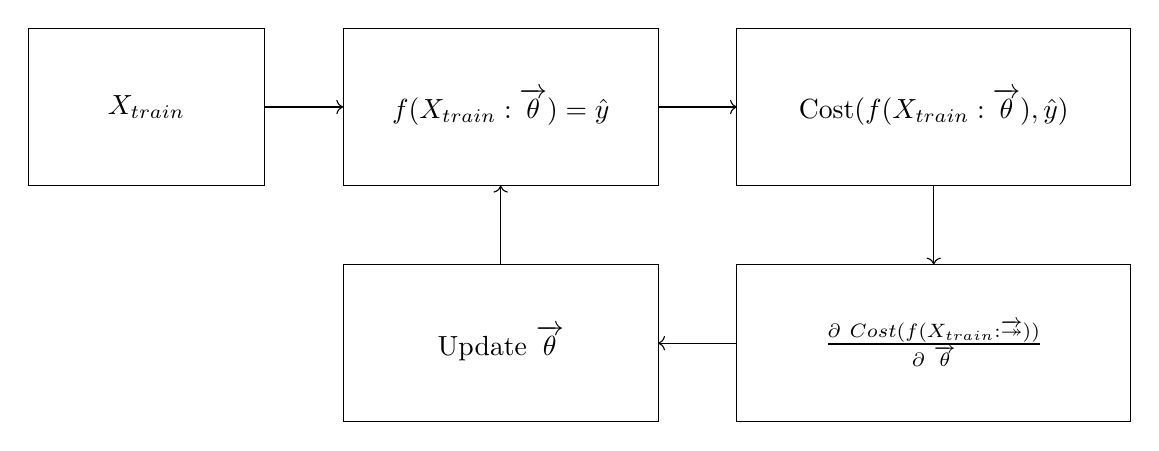
\begin{tikzpicture}
            \draw (0, 0) rectangle(3, 2);
            \draw (1.5, 1) node {$X_{train}$};

            \draw [->] (3, 1) -- (4, 1);

            \draw (4, 0) rectangle(8, 2);
            \draw (6, 1) node {$f(X_{train}: \overrightarrow{\theta}) = \hat{y}$};
            
            \draw [->] (8, 1) -- (9, 1);

            \draw (9, 0) rectangle(14, 2);
            \draw (11.5, 1) node {Cost($f(X_{train}: \overrightarrow{\theta}), \hat{y}$)};

            \draw [->] (11.5, 0) -- (11.5, -1);

            \draw (9, -1) rectangle(14, -3);
            \draw (11.5, -2) node {$\frac{\partial\ Cost(f(X_{train}: \overrightarrow{\twoheadrightarrow}))}{\partial\ \overrightarrow{\theta}}$};

            \draw [->] (9, -2) -- (8, -2);

            \draw (4, -1) rectangle(8, -3);
            \draw (6, -2) node {Update $\overrightarrow{\theta}$};

            \draw [->] (6, -1) -- (6, 0);

        \end{tikzpicture}

    \end{center}
\end{document}
